%% grundlagen.tex
%% $Id: grundlagen.tex 28 2007-01-18 16:31:32Z bless $
%%

\chapter{Grundlagen}
\label{ch:Grundlagen}
%% ==============================

%% ==============================
\section{Kryptographie mit öffentlichen Schlüsseln}
%% ==============================
\label{ch:Grundlagen:sec:PublicKeyCrypto}

\subsection{Prinzip}
\label{ch:Grundlagen:sec:PublicKeyCrypto:subsec:Prinzip}

\subsection{Authentisierung von Schlüsseln}
\label{ch:Grundlagen:sec:PublicKeyCrypto:subsec:KeyAuth}

\subsubsection{Zentrale PKI}
\label{ch:Grundlagen:sec:PublicKeyCrypto:subsec:KeyAuth:subsubsec:PKI}

\subsubsection{Web of Trust}
\label{ch:Grundlagen:sec:PublicKeyCrypto:subsec:KeyAuth:subsubsec:WOT}

\section{PGP/GnuPG}
\label{ch:Grundlagen:sec:PGP}

\subsection{Geschichte von PGP und GnuPG}
\label{ch:Grundlagen:sec:PGP:subsec:Geschichte}

\subsection{Eigenschaften/Fähigkeiten der Implementierungen}
\label{ch:Grundlagen:sec:PGP:subsec:Eigenschaften}

\subsection{Das GnuPG-Vertrauensmodell}
\label{sec:das-gnupg-vertrauensmodell}

bla bla bla

\begin{figure}[t]
  \centering
  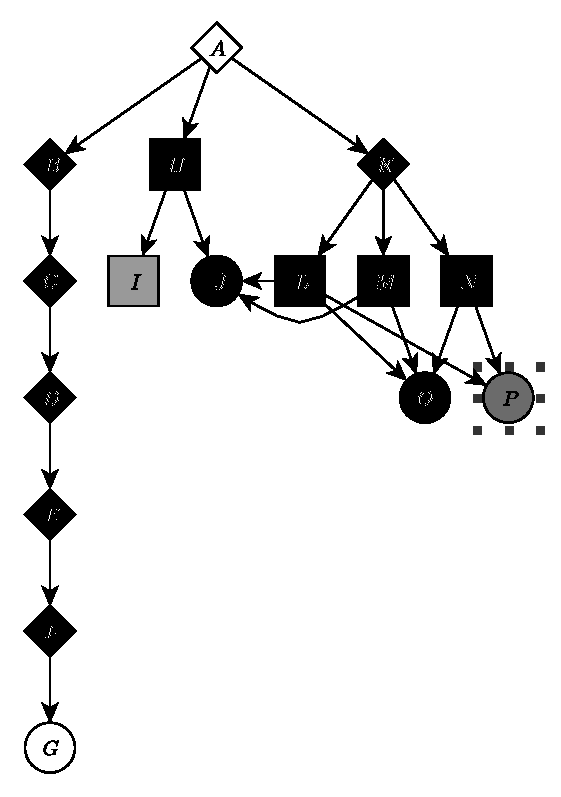
\includegraphics[scale=1.0]{images/trust-beispiel.pdf}
  \caption{Beispiel für die Berechnung der Gültigkeit von Schlüsseln}
  \label{fig:trust-beispiel}
\end{figure}

bla bla bla

\subsection{Soziale Komponente des Web of Trust}
\label{sec:sozi-komp-des}



%% ==============================
\section{Der OpenPGP-Standard (RFC4880)}
%% ==============================
\label{ch:Grundlagen:sec:OpenPGP}

\subsection{Paketformat v4}
\label{ch:Grundlagen:sec:OpenPGP:subsec:PaketFormat}

\subsection{Unterschiede v3}
\label{ch:Grundlagen:sec:OpenPGP:subsec:v3Format}

\section{Graphentheorie allgemein}
\label{ch:Grundlagen:sec:Graphentheorie}

\section{Netzwerkanalyse}
\label{ch:Grundlagen:sec:Netzwerkanalyse}

\subsection{Netzwerkstatistiken}
\label{ch:Grundlagen:sec:Netzwerkanalyse:subsec:Statistiken}

\subsection{Communities}
\label{ch:Grundlagen:sec:Netzwerkanalyse:subsec:Communities}

%% ==============================
\section{Verwandte Arbeiten}
%% ==============================
\label{ch:Grundlagen:sec:RelatedWork}

\subsection{Analysen des OpenPGP-Web of Trust}
\label{ch:Grundlagen:sec:RelatedWork:subsec:wot-analysis}

\subsection{Community-Strukturen allgemein}
\label{ch:Grundlagen:sec:RelatedWork:subsec:community-analysis}

%%% Local Variables: 
%%% mode: latex
%%% TeX-master: "diplarb"
%%% End: 
